\newpage\subsection{Architecture aléatoire}
\begin{figure}[h]
	\centering
		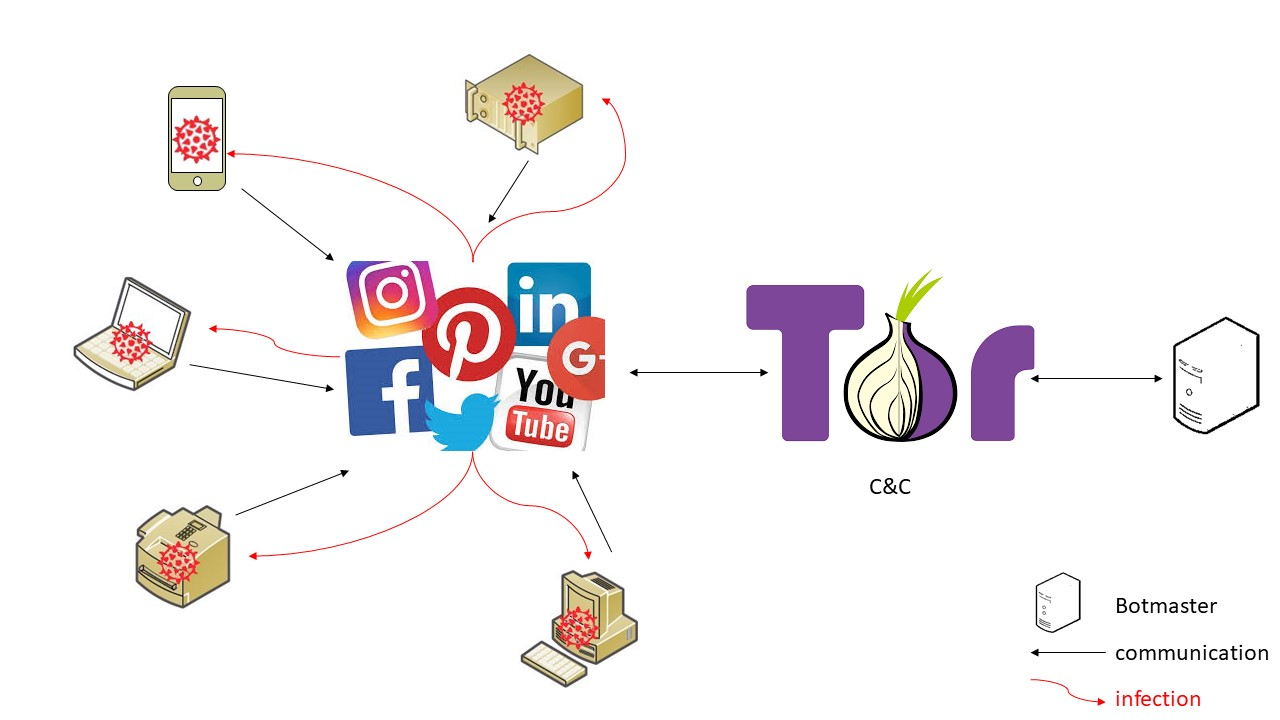
\includegraphics[width=0.75\textwidth]{reseau_aleatoire}
	\label{fig:réseau_aléatoire}
	\caption[Architecture aléatoire]{Architecture aléatoire}
\end{figure}
\subsubsection{Définition}
Ce concept représente une variante de l'architecture  centraliséee et peut se retrouver dans une variété de malware connue sous le nom de RATs\footnote{Remote Access Trojan}.Ces chevaux de Troie fonctionnent sur un principe de client/serveur parfois mis en place avec des techniques de social engineering (exemple: un fichier d'installation récupéré sur un site douteux). Ils exécutent la partie client à l'insu de l'utilisateur pour se connecter au serveur.
\newline Cette architecture tire profit de l'exploitation de plate-formes existantes supportant le protocole HTTP comme Facebook, Twitter, Yahoo, Evernote, Google, etc. et de réseau permettant de camoufler les échanges comme TOR, Hornet, etc.

\subsubsection {Liste des protocoles utilisés par le botnet}
\begin{itemize}
	\item HTTP
	\item protocole propriétaire (exemple XMPP\footnote{Extensible Messaging and Presence Protocol de MSN Messenger})
	\item IRC
\end{itemize}

\subsubsection{Avantages}
\begin{itemize}
	\item Architecture déjà existante
	\item Réseau important en terme d'utilisateurs
	\item Utilisation des canaux existants (exemple: messagerie instantanée)
	\item utilisation des fonctionnalités du réseau (exemple :Le réseau anonymisation TOR)
	\item Difficulté de démanteler son propre réseau
\end{itemize}

\subsubsection{Inconvénients}
\begin{itemize}
	\item Vulnérabilité du botnet face aux mécanismes de défense
	\item Connexion en permanence
	\item bloqué par le filtrage de liens de la plate-forme
\end{itemize}

%--------------------------------------------------------------------
%ajouter un botnet
%glisser le .csv dans le dossier exemples de la section 2
%inclure la ligne \csvautotabular[respect all]{Section/2-Ssection/exemples/nom-du-botnet}
%--------------------------------------------------------------------


\subsubsection{exemples}
\noindent
\resizebox{\textwidth}{!}{
\csvautotabular[respect all]{Section/2-Ssection/exemples/Cutwail.csv}
}
\resizebox{\textwidth}{!}{
\csvautotabular[respect all]{Section/2-Ssection/exemples/Carna.csv}
}